% Standalone TikZ source for the Glaukopis v21 template-generation → SFT flow.
% Compile with: pdflatex glaukopis_v21_flow.tex
\documentclass[tikz,border=6pt]{standalone}
\usepackage[T1]{fontenc}
\usetikzlibrary{arrows.meta,positioning,fit,backgrounds,calc,shapes.geometric}

\begin{document}
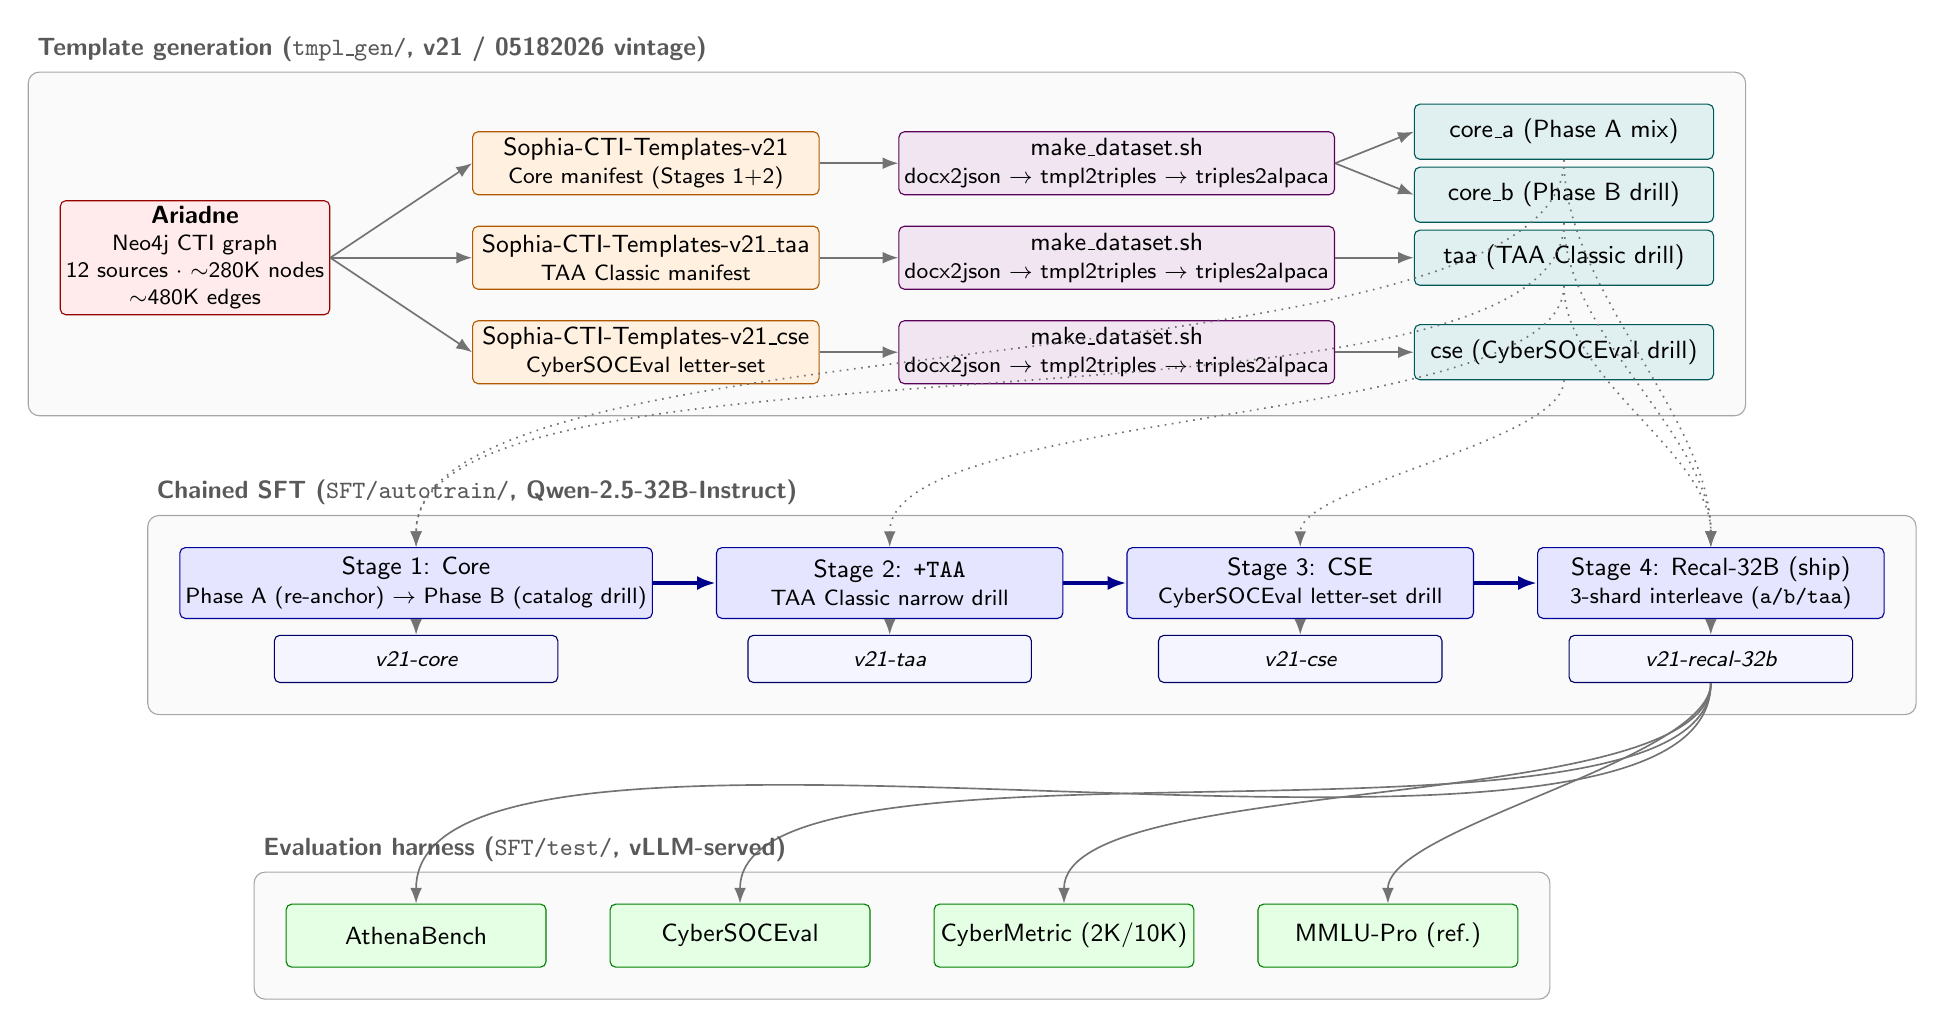
\begin{tikzpicture}[
    font=\sffamily\small,
    >={Latex[length=2.2mm]},
    node distance=4mm and 6mm,
    % Node styles
    src/.style    ={rectangle, rounded corners=2pt, draw=red!60!black, fill=red!8,
                    minimum width=33mm, minimum height=8mm, align=center, inner sep=2pt},
    tmpl/.style   ={rectangle, rounded corners=2pt, draw=orange!70!black, fill=orange!12,
                    minimum width=44mm, minimum height=8mm, align=center, inner sep=2pt},
    proc/.style   ={rectangle, rounded corners=2pt, draw=violet!70!black, fill=violet!10,
                    minimum width=50mm, minimum height=8mm, align=center, inner sep=2pt},
    shard/.style  ={rectangle, rounded corners=2pt, draw=teal!70!black, fill=teal!12,
                    minimum width=38mm, minimum height=7mm, align=center, inner sep=2pt},
    stage/.style  ={rectangle, rounded corners=2pt, draw=blue!60!black, fill=blue!10,
                    minimum width=44mm, minimum height=9mm, align=center, inner sep=2pt},
    ck/.style     ={rectangle, rounded corners=2pt, draw=blue!40!black, fill=blue!4,
                    minimum width=36mm, minimum height=6mm, align=center, inner sep=1pt,
                    font=\sffamily\footnotesize\itshape},
    bench/.style  ={rectangle, rounded corners=2pt, draw=green!50!black, fill=green!10,
                    minimum width=33mm, minimum height=8mm, align=center, inner sep=2pt},
    grp/.style    ={rectangle, rounded corners=4pt, draw=black!35, fill=black!2,
                    inner sep=4mm},
    grptitle/.style={font=\sffamily\bfseries\footnotesize, text=black!65},
    arr/.style    ={-{Latex[length=2mm]}, semithick, black!55},
    arrth/.style  ={-{Latex[length=2.4mm]}, line width=0.6mm, blue!55!black},
]

% -----------------------------------------------------------------------------
% Row 1: Ariadne CTI substrate (left) feeds three template manifests (right)
% -----------------------------------------------------------------------------
\node[src] (ariadne) {\textbf{Ariadne}\\[-0.3ex]\footnotesize Neo4j CTI graph\\[-0.3ex]\footnotesize 12 sources $\cdot$ $\sim$280K nodes\\[-0.3ex]\footnotesize $\sim$480K edges};

\node[tmpl, right=18mm of ariadne, yshift=12mm] (tcore) {Sophia-CTI-Templates-v21\\[-0.2ex]\footnotesize Core manifest (Stages 1+2)};
\node[tmpl, right=18mm of ariadne]              (ttaa)  {Sophia-CTI-Templates-v21\_taa\\[-0.2ex]\footnotesize TAA Classic manifest};
\node[tmpl, right=18mm of ariadne, yshift=-12mm](tcse)  {Sophia-CTI-Templates-v21\_cse\\[-0.2ex]\footnotesize CyberSOCEval letter-set};

\draw[arr] (ariadne.east) -- (tcore.west);
\draw[arr] (ariadne.east) -- (ttaa.west);
\draw[arr] (ariadne.east) -- (tcse.west);

% -----------------------------------------------------------------------------
% Row 2: make_dataset.sh pipeline (three pass-through pipelines)
% -----------------------------------------------------------------------------
\node[proc, right=10mm of tcore] (mcore) {make\_dataset.sh\\[-0.2ex]\footnotesize docx2json $\to$ tmpl2triples $\to$ triples2alpaca};
\node[proc, right=10mm of ttaa]  (mtaa)  {make\_dataset.sh\\[-0.2ex]\footnotesize docx2json $\to$ tmpl2triples $\to$ triples2alpaca};
\node[proc, right=10mm of tcse]  (mcse)  {make\_dataset.sh\\[-0.2ex]\footnotesize docx2json $\to$ tmpl2triples $\to$ triples2alpaca};

\draw[arr] (tcore.east) -- (mcore.west);
\draw[arr] (ttaa.east)  -- (mtaa.west);
\draw[arr] (tcse.east)  -- (mcse.west);

% -----------------------------------------------------------------------------
% Row 3: Seven dataset shards
% -----------------------------------------------------------------------------
\node[shard, right=10mm of mcore, yshift=4mm]  (score_a) {core\_a (Phase A mix)};
\node[shard, right=10mm of mcore, yshift=-4mm] (score_b) {core\_b (Phase B drill)};
\node[shard, right=10mm of mtaa]               (staa)    {taa (TAA Classic drill)};
\node[shard, right=10mm of mcse]               (scse)    {cse (CyberSOCEval drill)};

\draw[arr] (mcore.east) -- (score_a.west);
\draw[arr] (mcore.east) -- (score_b.west);
\draw[arr] (mtaa.east)  -- (staa.west);
\draw[arr] (mcse.east)  -- (scse.west);

% group all of the above as "Template generation"
\begin{pgfonlayer}{background}
  \node[grp,
        fit=(ariadne)(tcore)(tcse)(mcore)(mcse)(score_a)(score_b)(staa)(scse)
       ] (gG) {};
\end{pgfonlayer}
\node[grptitle, above=0mm of gG.north west, anchor=south west]
   {\sffamily\bfseries\small Template generation (\texttt{tmpl\_gen/}, v21 / 05182026 vintage)};

% -----------------------------------------------------------------------------
% Row 4: SFT four-stage chain — placed below the template-gen group
% -----------------------------------------------------------------------------
\node[stage, below=34mm of ariadne.south, anchor=west, xshift=-2mm] (S1)
   {Stage~1: Core\\[-0.2ex]\footnotesize Phase A (re-anchor) $\to$ Phase B (catalog drill)};
\node[stage, right=8mm of S1] (S2)
   {Stage~2: \texttt{+TAA}\\[-0.2ex]\footnotesize TAA Classic narrow drill};
\node[stage, right=8mm of S2] (S3)
   {Stage~3: CSE\\[-0.2ex]\footnotesize CyberSOCEval letter-set drill};
\node[stage, right=8mm of S3] (S4)
   {Stage~4: Recal-32B (ship)\\[-0.2ex]\footnotesize 3-shard interleave (\texttt{a/b/taa})};

\node[ck, below=2mm of S1] (C1) {v21-core};
\node[ck, below=2mm of S2] (C2) {v21-taa};
\node[ck, below=2mm of S3] (C3) {v21-cse};
\node[ck, below=2mm of S4] (C4) {v21-recal-32b};

\draw[arrth] (S1.east) -- (S2.west);
\draw[arrth] (S2.east) -- (S3.west);
\draw[arrth] (S3.east) -- (S4.west);
\draw[arr] (S1.south) -- (C1.north);
\draw[arr] (S2.south) -- (C2.north);
\draw[arr] (S3.south) -- (C3.north);
\draw[arr] (S4.south) -- (C4.north);

% group as "SFT chain"
\begin{pgfonlayer}{background}
  \node[grp,
        fit=(S1)(S4)(C1)(C4)
       ] (gS) {};
\end{pgfonlayer}
\node[grptitle, above=0mm of gS.north west, anchor=south west]
   {\sffamily\bfseries\small Chained SFT (\texttt{SFT/autotrain/}, Qwen-2.5-32B-Instruct)};

% -----------------------------------------------------------------------------
% Shard → Stage edges (light, to keep readable)
% -----------------------------------------------------------------------------
\draw[arr, dotted] (score_a.south) to[out=-90,in=90,looseness=0.5] (S1.north);
\draw[arr, dotted] (score_b.south) to[out=-90,in=90,looseness=0.5] (S1.north);
\draw[arr, dotted] (staa.south)    to[out=-90,in=90,looseness=0.5] (S2.north);
\draw[arr, dotted] (scse.south)    to[out=-90,in=90,looseness=0.5] (S3.north);
\draw[arr, dotted] (score_a.south) to[out=-90,in=90,looseness=0.8] (S4.north);
\draw[arr, dotted] (score_b.south) to[out=-90,in=90,looseness=0.8] (S4.north);
\draw[arr, dotted] (staa.south)    to[out=-90,in=90,looseness=0.8] (S4.north);

% -----------------------------------------------------------------------------
% Row 5: evaluation harness
% -----------------------------------------------------------------------------
\node[bench, below=28mm of C1.south] (B1) {AthenaBench};
\node[bench, right=8mm of B1] (B2) {CyberSOCEval};
\node[bench, right=8mm of B2] (B3) {CyberMetric (2K/10K)};
\node[bench, right=8mm of B3] (B4) {MMLU-Pro (ref.)};

\draw[arr] (C4.south) to[out=-90,in=90,looseness=0.5] (B1.north);
\draw[arr] (C4.south) to[out=-90,in=90,looseness=0.5] (B2.north);
\draw[arr] (C4.south) to[out=-90,in=90,looseness=0.5] (B3.north);
\draw[arr] (C4.south) to[out=-90,in=90,looseness=0.5] (B4.north);

\begin{pgfonlayer}{background}
  \node[grp,
        fit=(B1)(B4)
       ] (gE) {};
\end{pgfonlayer}
\node[grptitle, above=0mm of gE.north west, anchor=south west]
   {\sffamily\bfseries\small Evaluation harness (\texttt{SFT/test/}, vLLM-served)};

\end{tikzpicture}
\end{document}
